\documentclass{standalone}
\usepackage{calc}
\usepackage{xparse}
\usepackage{tikz}
\usetikzlibrary{patterns,calc,arrows,arrows.meta,angles,quotes}
\usetikzlibrary{decorations.pathreplacing,calligraphy,babel}
\usepackage[framemethod=tikz]{mdframed}
\usepackage[caption=false,font=footnotesize]{subfig}
\tikzset{%
  point/.style={circle,inner sep=1.25pt,minimum size=1.25pt,draw,fill=#1},
  point/.default=red
}
\definecolor{c0}{rgb}{0.2,0.4,0.67}
\definecolor{c1}{rgb}{0.67,0.4,0.12}
\definecolor{c2}{rgb}{0.53,0.6,0.13}
\definecolor{c3}{rgb}{0.53,0.53,0.4}
\NewDocumentCommand\witness{mmmO{c2}}{%
  \node[point=#4] (w0) at (#1) {};
  \node[point=#4] (w1) at (#2) {};
  \node[point=#4] (w2) at (#3) {};
  \draw[#4] (w0)--(w1)--(w2);
}
\def\myWitness{\witness{0,0}{\x,\y}{\dc,0}}
\NewDocumentCommand\crvb{}{%
  \def\a{-0.618034}
  \def\b{-1.61803}
  \def\c{.52573}
  \def\s{.85065}
  \draw[c1,parametric,variable=\t,smooth,
    domain=1:2.6,
    samples=60]
  plot
  ({\a*cos(\t r)*\c-\b*sin(\t r)*\s},{\a*cos(\t r)*\s+\b*sin(\t r)*\c});
}
\NewDocumentCommand\sights{O{a}O{b}O{c}O{c2}}{%
  \node[point=#4] (#1) at (0,1) {};
  \node[point=#4] (#2) at (1,0) {};
  \node[point=#4] (#3) at (1,1) {};
  \draw[#4] (#1)--(#2)--(#3);
}
\NewDocumentCommand\elipricArc{mm}{
  \draw[c1,thick] ($(0, 0) + (0:#1 cm and #2 cm)$(P) arc (0:90:#1 cm and #2 cm);
}
\NewDocumentCommand\crv{}{%
  \begin{scope}[shift={(1,-1)},rotate=270]\coordinate (q1) at (1,0);\end{scope}
  \begin{scope}[shift={(1.06,-.721)},rotate=250]\coordinate (q2) at (1,0);\end{scope}
  \begin{scope}[shift={(1.2929,-.5858)},rotate=225]\coordinate (q3) at (1,0);\end{scope}
  \begin{scope}[shift={(1.655,-.717)},rotate=200]\coordinate (q4) at (1,0);\end{scope}
  \begin{scope}[shift={(2,-1)},rotate=180]\coordinate (q5) at (1,0);\end{scope}
  \draw [c1] plot [smooth] coordinates {(q1)(q2)(q3)(q4)(q5)};
}
\NewDocumentCommand\obs{}{%
  \coordinate (q0) at (0.76,0.1);
  \coordinate (q1) at (3.05,0.1);
  \coordinate (q2) at (3.05,0.2);
  \coordinate (q3) at (0.76,0.2);
  \filldraw[fill=white,draw=c0] (q0) -- (q1) -- (q2) -- (q3) -- cycle;%
  \node[point=c0] at (q0) {};
  \node[point=c0] at (q1) {};
  \node[point=c0] at (q2) {};
  \node[point=c0] at (q3) {};
}
\NewDocumentCommand\witnessB{O{a}O{b}O{c}O{c2}}{%
  \node[point=#4] (#1) at (0,1) {};
  \node[point=#4] (#2) at (1,0) {};
  \node[point=#4] (#3) at (1,1) {};
  \draw[#4] (#1)--(#2)--(#3);
}
\begin{document}
%\tikzset{every picture/.append style={scale=1}}%\scriptsize
\begin{tabular}{cccccc}
  \multicolumn{2}{c}{\input{square1/square1.tex}} &
  \multicolumn{2}{c}{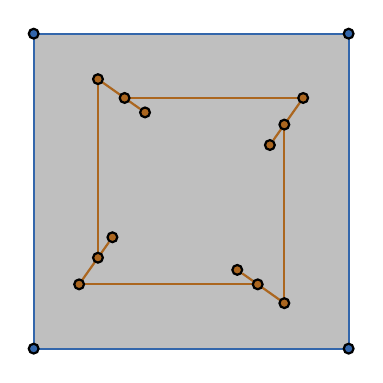
\begin{tikzpicture}[thick]
  % Boundary
  \coordinate (b0) at (-2,-2);
  \coordinate (b1) at (2,-2);
  \coordinate (b2) at (2,2);
  \coordinate (b3) at (-2,2);
  \filldraw[fill=lightgray,draw=c0] (b0) -- (b1) -- (b2) -- (b3) -- cycle;
  \node[point=c0] at (b0) {};
  \node[point=c0] at (b1) {};
  \node[point=c0] at (b2) {};
  \node[point=c0] at (b3) {};
  % Solution segments
  \pgfmathparse{1}\let\da\pgfmathresult
  \pgfmathparse{sqrt(2)}\let\db\pgfmathresult
  \pgfmathparse{pi*0.5}\let\angle\pgfmathresult
  \pgfmathparse{cos(deg(\angle))}\let\c\pgfmathresult
  \pgfmathparse{sqrt(\da*\da+\db*\db-2*\c*\da*\db)}\let\dc\pgfmathresult
  \pgfmathparse{(\dc*\dc-\db*\db+\da*\da)/(2*\dc)}\let\x\pgfmathresult
  \pgfmathparse{sqrt(\da*\da-\x*\x)}\let\y\pgfmathresult
  %
  \coordinate[shift={(-2,-2)}] (a0) at (\x,\y);
  \coordinate[shift={(2-\dc,-2)}] (a1) at (\x,\y);
  \begin{scope}[rotate=90,shift={(-2,-2)}]\coordinate (a2) at (\x,\y);\end{scope}
  \begin{scope}[rotate=90,shift={(2-\dc,-2)}]\coordinate (a3) at (\x,\y);\end{scope}
  \begin{scope}[rotate=180,shift={(-2,-2)}]\coordinate (a4) at (\x,\y);\end{scope}
  \begin{scope}[rotate=180,shift={(2-\dc,-2)}]\coordinate (a5) at (\x,\y);\end{scope}
  \begin{scope}[rotate=270,shift={(-2,-2)}]\coordinate (a6) at (\x,\y);\end{scope}
  \begin{scope}[rotate=270,shift={(2-\dc,-2)}]\coordinate (a7) at (\x,\y);\end{scope}
  \draw[c1] (a0)--(a1);
  \draw[c1] (a2)--(a3);
  \draw[c1] (a4)--(a5);
  \draw[c1] (a6)--(a7);
  \node[point=c1,shift={(-2,-2)}] (a8) at (\da,\db) {};
  \draw[c1] (a0)--(a8);
  \begin{scope}[rotate=90,shift={(-2,-2)}]\node[point=c1] (a9) at (\da,\db) {};\end{scope}
  \draw[c1] (a2)--(a9);
  \begin{scope}[rotate=180,shift={(-2,-2)}]\node[point=c1] (a10) at (\da,\db) {};\end{scope}
  \draw[c1] (a4)--(a10);
  \begin{scope}[rotate=270,shift={(-2,-2)}]\node[point=c1] (a11) at (\da,\db) {};\end{scope}
  \draw[c1] (a6)--(a11);
  % Witnesses
  \begin{scope}[shift={(-2,-2)}]\myWitness\end{scope}
  \begin{scope}[shift={(2-\dc,-2)}]\myWitness\end{scope}
  \begin{scope}[shift={(-2,-2+\dc)},rotate=270]\myWitness\end{scope}
  \begin{scope}[shift={(-2,-2+\db)},rotate=305]\myWitness\end{scope}
  %%
  %% \begin{scope}[shift={(1,-1)},rotate=270]\witness[p1][q1][r1][c2!20!black]\end{scope}
  %% \begin{scope}[shift={(1.06,-.721)},rotate=250]\witness[p2][q2][r2][c2!40!black]\end{scope}
  %% \begin{scope}[shift={(1.2929,-.5858)},rotate=225]\witness[p3][q3][r3][c2!60!black]\end{scope}
  %% \begin{scope}[shift={(1.655,-.717)},rotate=200]\witness[p4][q4][r4][c2!80!black]\end{scope}
  %% \begin{scope}[shift={(2,-1)},rotate=180]\witness[p5][q5][r5][c2!100!black]\end{scope}
  %% %%
  %% \begin{scope}[shift={(-2,2)},rotate=0]\crvb\end{scope}
  %% \begin{scope}[shift={(-2,-2)},rotate=90]\crvb\end{scope}
  %% \begin{scope}[shift={(2,-2)},rotate=180]\crvb\end{scope}
  %% \begin{scope}[shift={(2,2)},rotate=270]\crvb\end{scope}
  %% %%
  \node[point=c1] (n0) at (a0) {};
  \node[point=c1] (n1) at (a1) {};
  \node[point=c1] (n2) at (a2) {};
  \node[point=c1] (n3) at (a3) {};
  \node[point=c1] (n4) at (a4) {};
  \node[point=c1] (n5) at (a5) {};
  \node[point=c1] (n6) at (a6) {};
  \node[point=c1] (n7) at (a7) {};
\end{tikzpicture}
} &
  \multicolumn{2}{c}{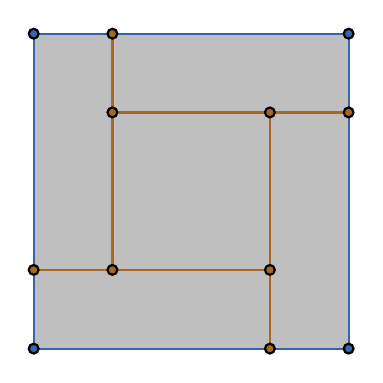
\begin{tikzpicture}[thick]
  \coordinate (p0) at (-2,-2);
  \coordinate (p1) at (2,-2);
  \coordinate (p2) at (2,2);
  \coordinate (p3) at (-2,2);
  \filldraw[fill=lightgray,draw=c0] (p0) -- (p1) -- (p2) -- (p3) -- cycle;%
  \node[point=c0] (m0) at (p0) {};
  \node[point=c0] at (p1) {};
  \node[point=c0] at (p2) {};
  \node[point=c0] at (p3) {};
  \coordinate (a0) at (-2,-1);
  \coordinate (a1) at (1,-1);
  \coordinate (a2) at (1,-2);
  \coordinate (a3) at (1,1);
  \coordinate (a4) at (2,1);
  \coordinate (a5) at (-1,1);
  \coordinate (a6) at (-1,2);
  \coordinate (a7) at (-1,-1);
  \draw[c1] (a0)--(a1);
  \draw[c1] (a2)--(a3);
  \draw[c1] (a4)--(a5);
  \draw[c1] (a6)--(a7);
  %%%
  \begin{scope}[shift={(-1.3,1)}]\sights\end{scope}
  \begin{scope}[shift={(-1,0.5)},rotate=90]\sights\end{scope}
  \begin{scope}[shift={(-1,-1.3)},rotate=90]\sights\end{scope}
  %%
  \begin{scope}[shift={(1,-1)},rotate=270]\sights[p1][q1][r1][c2!20!black]\end{scope}
  \begin{scope}[shift={(1.06,-.721)},rotate=250]\sights[p2][q2][r2][c2!40!black]\end{scope}
  \begin{scope}[shift={(1.2929,-.5858)},rotate=225]\sights[p3][q3][r3][c2!60!black]\end{scope}
  \begin{scope}[shift={(1.655,-.717)},rotate=200]\sights[p4][q4][r4][c2!80!black]\end{scope}
  \begin{scope}[shift={(2,-1)},rotate=180]\sights[p5][q5][r5][c2!100!black]\end{scope}
  %%
  %% \draw plot [smooth] coordinates {(q1)(q2)(q3)(q4)(q5)};
  %% \begin{scope}[shift={(0,0)},rotate=0]\crv\end{scope}
  %% \begin{scope}[shift={(-3,-2)},rotate=90]\crvb\end{scope}
  %% \begin{scope}[shift={(0,0)},rotate=180]\crvb\end{scope}
  %% \begin{scope}[shift={(3,2)},rotate=270]\crvb\end{scope}
  \begin{scope}[shift={(-2,2)},rotate=0]\crvb\end{scope}
  \begin{scope}[shift={(-2,-2)},rotate=90]\crvb\end{scope}
  \begin{scope}[shift={(2,-2)},rotate=180]\crvb\end{scope}
  \begin{scope}[shift={(2,2)},rotate=270]\crvb\end{scope}
  %%
  \node[point=c1] (n0) at (a0) {};
  \node[point=c1] (n1) at (a1) {};
  \node[point=c1] (n2) at (a2) {};
  \node[point=c1] (n3) at (a3) {};
  \node[point=c1] (n4) at (a4) {};
  \node[point=c1] (n5) at (a5) {};
  \node[point=c1] (n6) at (a6) {};
  \node[point=c1] (n7) at (a7) {};
\end{tikzpicture}
}\\
  \multicolumn{2}{c}{$d_1 = 1$, $d_2 = 1$, $\alpha = 90^{\circ}$} &
  \multicolumn{2}{c}{$d_1 = 1$, $d_2 = \sqrt{2}$, $\alpha = 90^{\circ}$} &
  \multicolumn{2}{c}{$d_1 = 1$, $d_2 = \sqrt{2}$, $\alpha = 45^{\circ}$}\\
  \multicolumn{3}{c}{\hspace{44pt}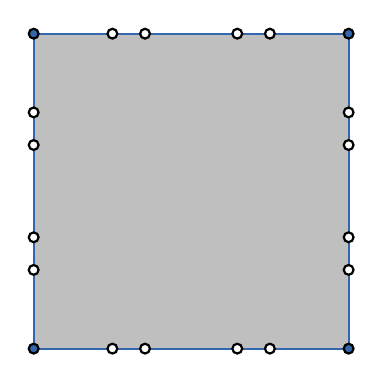
\begin{tikzpicture}[thick]
  % Boundary
  \coordinate (b0) at (-2,-2);
  \coordinate (b1) at (2,-2);
  \coordinate (b2) at (2,2);
  \coordinate (b3) at (-2,2);
  \filldraw[fill=lightgray,draw=c0] (b0) -- (b1) -- (b2) -- (b3) -- cycle;
  \node[point=c0] at (b0) {};
  \node[point=c0] at (b1) {};
  \node[point=c0] at (b2) {};
  \node[point=c0] at (b3) {};
  \begin{scope}[rotate=0,shift={(-2,-2)}]
    \elipricArc{1.4142}{1}
    \elipricArc{1}{1.4142}
    \node[point=white] at (0,1.4142) {};
    \node[point=white] at (1.4142,0) {};
    \node[point=white] at (0,1) {};
    \node[point=white] at (1,0) {};
  \end{scope}
  \begin{scope}[rotate=90,shift={(-2,-2)}]
    \elipricArc{1.4142}{1}
    \elipricArc{1}{1.4142}
    \node[point=white] at (0,1.4142) {};
    \node[point=white] at (1.4142,0) {};
    \node[point=white] at (0,1) {};
    \node[point=white] at (1,0) {};
  \end{scope}
  \begin{scope}[rotate=180,shift={(-2,-2)}]
    \elipricArc{1.4142}{1}
    \elipricArc{1}{1.4142}
    \node[point=white] at (0,1.4142) {};
    \node[point=white] at (1.4142,0) {};
    \node[point=white] at (0,1) {};
    \node[point=white] at (1,0) {};
  \end{scope}
  \begin{scope}[rotate=270,shift={(-2,-2)}]
    \elipricArc{1.4142}{1}
    \elipricArc{1}{1.4142}
    \node[point=white] at (0,1.4142) {};
    \node[point=white] at (1.4142,0) {};
    \node[point=white] at (0,1) {};
    \node[point=white] at (1,0) {};
  \end{scope}
  \pgfmathparse{2.4142}\let\dc\pgfmathresult
  \pgfmathparse{1}\let\x\pgfmathresult
  \pgfmathparse{0}\let\y\pgfmathresult
  \begin{scope}[rotate=-10,shift={(-1.694,-1.905)}]\myWitness\end{scope}
\end{tikzpicture}
} &
  \multicolumn{3}{c}{\hspace{8pt}\begin{tikzpicture}[]
  \coordinate (p0) at (-2,-2);
  \coordinate (p1) at (2,-2);
  \coordinate (p2) at (2,2);
  \coordinate (p3) at (-2,2);
  \filldraw[fill=lightgray,draw=c0] (p0) -- (p1) -- (p2) -- (p3) -- cycle;%
  \node[point=c0] at (p0) {};
  \node[point=c0] at (p1) {};
  \node[point=c0] at (p2) {};
  \node[point=c0] at (p3) {};
  %
  \begin{scope}[shift={(-2,-2)},rotate=0]\obs\end{scope}
  \begin{scope}[shift={(2,-2)},rotate=90]\obs\end{scope}
  \begin{scope}[shift={(2,2)},rotate=180]\obs\end{scope}
  \begin{scope}[shift={(-2,2)},rotate=270]\obs\end{scope}
  %
  \coordinate (r0) at (-0.95,-0.95);
  \coordinate (r1) at (0.95,-0.95);
  \coordinate (r2) at (0.95,0.95);
  \coordinate (r3) at (-0.95,0.95);
  \filldraw[fill=white,draw=c0] (r0) -- (r1) -- (r2) -- (r3) -- cycle;%
  \node[point=c0] at (q0) {};
  \node[point=c0] at (q1) {};
  \node[point=c0] at (q2) {};
  \node[point=c0] at (q3) {};
  %%% Witnesses
  \begin{scope}[shift={(-0.586,-1.293)},rotate=135]\witnessB\end{scope}
  \begin{scope}[shift={(-0.592,-1.234)},rotate=140]\witnessB\end{scope}
  \node[point=c1] at (b) {};
  \begin{scope}[rotate=90]
    \begin{scope}[shift={(-0.592,-1.234)},rotate=140]\node[point=c1] at (1,0) {};\end{scope}
  \end{scope}
  \begin{scope}[rotate=180]
    \begin{scope}[shift={(-0.592,-1.234)},rotate=140]\node[point=c1] at (1,0) {};\end{scope}
  \end{scope}
  \begin{scope}[rotate=270]
    \begin{scope}[shift={(-0.592,-1.234)},rotate=140]\node[point=c1] at (1,0) {};\end{scope}
  \end{scope}
  %
  \begin{scope}[shift={(-0.601,-1.399)},rotate=127]\witnessB\end{scope}
  \node[point=c1] at (b) {};
  \begin{scope}[rotate=90]
    \begin{scope}[shift={(-0.601,-1.399)},rotate=127]\node[point=c1] at (1,0) {};\end{scope}
  \end{scope}
  \begin{scope}[rotate=180]
    \begin{scope}[shift={(-0.601,-1.399)},rotate=127]\node[point=c1] at (1,0) {};\end{scope}
  \end{scope}
  \begin{scope}[rotate=270]
    \begin{scope}[shift={(-0.601,-1.399)},rotate=127]\node[point=c1] at (1,0) {};\end{scope}
  \end{scope}
  %% Solution
  \begin{scope}[shift={(-2,2)},rotate=0]\crvb\end{scope}
  \begin{scope}[shift={(-2,-2)},rotate=90]\crvb\end{scope}
  \begin{scope}[shift={(2,-2)},rotate=180]\crvb\end{scope}
  \begin{scope}[shift={(2,2)},rotate=270]\crvb\end{scope}
  %%
\end{tikzpicture}
}\\
  \multicolumn{3}{c}{\hspace{44pt}$d_1 = 1$, $d_2 = \sqrt{2}$, $\alpha = 180^{\circ}$} &
  \multicolumn{3}{c}{\hspace{8pt}$d_1 = 1$, $d_2 = \sqrt{2}$, $\alpha = 45^{\circ}$}
  %% \multicolumn{6}{p{\linewidth}}{The free space is filled with a light-gray
  %%   color. The boundary of the free space is drawn with blue segments.
  %%   Orange curves contains all the possible locations of the sensor.
  %%   A pair of green segments with a common endpoint shows a witness.}
\end{tabular}
\end{document}
